\section{Çok Amaçlı Optimizasyon}
Yapısal sistemlerin optimizasyonunda zaman zaman birbiriyle çelişen birden fazla amacın eş zamanlı olarak optimize edilmesi gerekebilir. Bu bölümde, çok amaçlı optimizasyon yöntemleri ve uygulamaları incelenecektir. \sidenote{Çok amaçlı optimizasyonda, tek bir optimal çözüm yerine Pareto-optimal çözümler kümesi elde edilir.
Çok amaçlı optimizasyonun daha iyi anlaşılması için bağlantıdaki örnek kod incelenebilir.


\qrcode[height=1in]{https://github.com/btayfur/structural-optimization/blob/main/Code/Examples/Exmp5/}}

\subsection{Çok Amaçlı Optimizasyonun Temelleri}
Birden fazla amaç fonksiyonunun eş zamanlı optimizasyonu:

\begin{tcolorbox}[title=Temel Kavramlar]
\begin{itemize}
    \item \textbf{Pareto Optimallik:} Baskın çözümler
    \item \textbf{Trade-off:} Amaçlar arası ödünleşim
    \item \textbf{Karar Verme:} Çözüm seçimi
    \item \textbf{Ağırlıklandırma:} Amaçların önceliklendirilmesi
\end{itemize}
\end{tcolorbox}

\subsection{Matematiksel Formülasyon}
Çok amaçlı optimizasyon probleminin genel yapısı:

\begin{equation}
\begin{aligned}
& \text{minimize} & & \mathbf{F}(\mathbf{x}) = [f_1(\mathbf{x}), f_2(\mathbf{x}), \ldots, f_k(\mathbf{x})]^T \\
& \text{subject to} & & g_i(\mathbf{x}) \leq 0, & & i = 1,\ldots,m \\
& & & h_j(\mathbf{x}) = 0, & & j = 1,\ldots,p \\
& & & \mathbf{x}^L \leq \mathbf{x} \leq \mathbf{x}^U
\end{aligned}
\end{equation}




\begin{marginfigure}
\centering
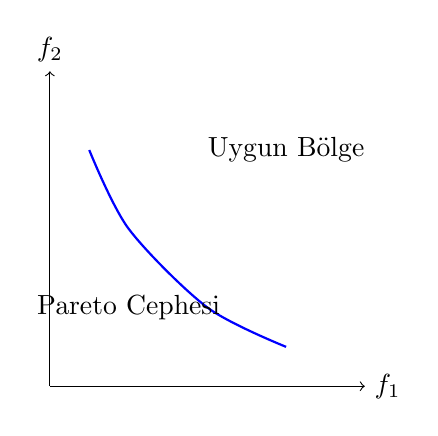
\begin{tikzpicture}
\draw[->] (0,0) -- (4,0) node[right] {$f_1$};
\draw[->] (0,0) -- (0,4) node[above] {$f_2$};
\draw[blue,thick] plot[smooth] coordinates {(0.5,3) (1,2) (2,1) (3,0.5)};
\node at (3,3) {Uygun Bölge};
\node at (1,1) {Pareto Cephesi};
\end{tikzpicture}
\caption{Pareto cephesi örneği}
\end{marginfigure}

\subsection{Çözüm Yaklaşımları}
Çok amaçlı optimizasyon problemlerinin çözümünde kullanılan temel stratejilerin incelenmesi, problemi ele alış biçimine göre farklı yaklaşımlar sunar. Yani esas olarak burada karar verici mühendisin kendisidir. Amaç fonksiyonlarının birbirlerine kıyasla üstün olup olmaması veya oransallığı bu kararda ve seçilecek stratejide etkilidir.

\subsubsection{Skalerleştirme Yöntemleri}
Çok amaçlı optimizasyon problemini tek amaçlı probleme dönüştüren yaklaşımlardır. Bu yöntemler, çoklu amaçları birleştirerek problemi daha kolay çözülebilir hale getirir. Skalerleştirme yöntemleri, hızlı ve kolay uygulanabilir olmaları nedeniyle mühendislik problemlerinde yaygın olarak kullanılır. Ancak uygun ağırlıkların belirlenmesi, çözümün kalitesini doğrudan etkilediği için süreci zorlaştırabilir.

\begin{tcolorbox}[title=Yaygın Skalerleştirme Yöntemleri]
\begin{itemize}
    \item \textbf{Ağırlıklı Toplam Yöntemi:} $F(x) = \sum_{i=1}^{k} w_i f_i(x)$
    \item \textbf{$\varepsilon$-Kısıt Yöntemi:} Bir amaç optimize edilirken diğerleri kısıt olarak tanımlanır
    \item \textbf{Hedef Programlama:} $\min \sum_{i=1}^{k} w_i |f_i(x) - T_i|$ (burada $T_i$ hedef değerlerdir)
\end{itemize}
\end{tcolorbox}

\subsubsection{Pareto Tabanlı Yaklaşımlar}
Pareto tabanlı yaklaşımlar, tüm Pareto-optimal çözümleri veya bunların iyi bir temsilini bulmayı hedefler. Bu yöntemler, çözüm uzayının daha geniş bir bölümünü keşfetmeyi sağlar ve karar vericiye daha fazla alternatif sunar. Pareto tabanlı yaklaşımlar, özellikle evrimsel algoritmaların kullanıldığı durumlarda daha etkilidir.

Pareto tabanlı yaklaşımların temel bileşenleri şunlardır:
\begin{itemize}
    \item \textbf{Baskınlık İlişkisi:} Bir çözümün diğerine göre daha iyi olup olmadığının belirlenmesi
    \item \textbf{Çeşitlilik Mekanizmaları:} Pareto cephesi boyunca çözümlerin homojen dağılmasını sağlayan teknikler
    \item \textbf{Elit Stratejiler:} İyi çözümlerin korunmasını sağlayan mekanizmalar
\end{itemize}

\begin{marginfigure}
\centering
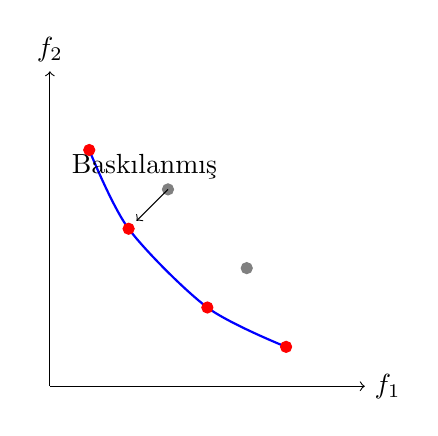
\begin{tikzpicture}
\draw[->] (0,0) -- (4,0) node[right] {$f_1$};
\draw[->] (0,0) -- (0,4) node[above] {$f_2$};
\draw[blue,thick] plot[smooth] coordinates {(0.5,3) (1,2) (2,1) (3,0.5)};
\filldraw[red] (0.5,3) circle (2pt);
\filldraw[red] (1,2) circle (2pt);
\filldraw[red] (2,1) circle (2pt);
\filldraw[red] (3,0.5) circle (2pt);
\filldraw[gray] (1.5,2.5) circle (2pt);
\filldraw[gray] (2.5,1.5) circle (2pt);
\draw[->] (1.5,2.5) -- (1.1,2.1);
\node at (1.2,2.8) {Baskılanmış};
\end{tikzpicture}
\caption{Pareto baskınlık kavramı}
\end{marginfigure}

\subsubsection{İnteraktif Yöntemler}
İnteraktif yöntemler, karar vericiyi optimizasyon sürecine dahil ederek, tercihlerine göre çözüm uzayını daraltır. Bu yaklaşım, karar vericinin bilgi ve deneyimini algoritmanın çalışmasına entegre eder. İnteraktif yöntemler, özellikle karmaşık mühendislik problemlerinde, uzman bilgisinin çözüm sürecine dahil edilmesi açısından değerlidir.

İnteraktif yaklaşımların avantajları:
\begin{itemize}
    \item Karar vericinin tercihlerini doğrudan sürece yansıtabilme
    \item Hesaplama kaynaklarını ilgi duyulan çözüm bölgesine yönlendirme
    \item Daha anlamlı ve uygulanabilir sonuçlar elde etme
\end{itemize}

\subsection{Evrimsel Çok Amaçlı Optimizasyon Algoritmaları}
Evrimsel algoritmaların çok amaçlı optimizasyon problemlerine uygulanması, klasik yöntemlere göre önemli avantajlar sağlar. Bu algoritmalar, tek seferde birden fazla çözüm üretebilme, karmaşık amaç fonksiyonlarını ele alabilme ve geniş çözüm uzaylarını etkili bir şekilde tarayabilme özellikleriyle öne çıkar.

\subsubsection{NSGA-II (Non-dominated Sorting Genetic Algorithm)}
NSGA-II, çok amaçlı evrimsel optimizasyon alanında en yaygın kullanılan algoritmalardan biridir. Baskınlık sıralama ve yoğunluk mesafesi hesaplama mekanizmalarıyla, hem Pareto-optimal çözümlere yakınsama hem de çözümler arasında çeşitlilik sağlar. NSGA-II, $O(MN^2)$ hesaplama karmaşıklığıyla oldukça verimli çalışır ve birçok mühendislik probleminde başarıyla uygulanmıştır.

NSGA-II'nin temel bileşenleri:
\begin{itemize}
    \item \textbf{Hızlı Baskınlık Sıralama:} Popülasyondaki çözümleri baskınlık ilişkisine göre sıralar
    \item \textbf{Yoğunluk Mesafesi:} Aynı baskınlık seviyesindeki çözümler arasında çeşitliliği korur
    \item \textbf{İkili Turnuva Seçimi:} Baskınlık seviyesi ve yoğunluk mesafesine dayalı seçim mekanizması
\end{itemize}


\subsubsection{MOEA/D (Multiobjective Evolutionary Algorithm based on Decomposition)}
MOEA/D, çok amaçlı optimizasyon problemini bir dizi tek amaçlı alt probleme ayrıştırarak çözen bir evrimsel algoritmadır. Her alt problem, komşu alt problemlerle bilgi paylaşımı yaparak eş zamanlı olarak optimize edilir. Bu yaklaşım, özellikle çok sayıda amaç fonksiyonu içeren problemlerde etkilidir ve hesaplama açısından verimlidir.

MOEA/D'nin avantajları:
\begin{itemize}
    \item Komşuluk yapısı sayesinde etkili bilgi paylaşımı
    \item Çok sayıda amaç fonksiyonu içeren problemlere uygunluk
    \item Farklı ayrıştırma yöntemlerinin kullanılabilmesi (Tchebycheff, ağırlıklı toplam vb.)
\end{itemize}

\subsubsection{SPEA2 (Strength Pareto Evolutionary Algorithm)}
SPEA2, sabit büyüklükte bir arşiv kullanarak Pareto-optimal çözümleri saklayan ve rafine eden bir evrimsel algoritmadır. Algoritma, her çözüme bir uygunluk değeri atayarak hem baskınlık ilişkisini hem de çözüm yoğunluğunu dikkate alır. SPEA2, özellikle çeşitlilik ve yakınsama arasında iyi bir denge kurması nedeniyle tercih edilir.

SPEA2'nin önemli özellikleri:
\begin{itemize}
    \item \textbf{Güç Değeri:} Bir çözümün kaç çözümü baskıladığını ölçer
    \item \textbf{Yoğunluk Tahmini:} K-en yakın komşu yöntemiyle hesaplanır
    \item \textbf{Harici Arşiv:} Pareto-optimal çözümleri etkin bir şekilde depolar ve günceller
\end{itemize}

\subsection{Karar Verme Süreçleri}
Çok amaçlı optimizasyon, bir dizi Pareto-optimal çözüm üretir ve bu çözümler arasından seçim yapılması gerekir. Karar verme süreci, optimizasyon sürecinin kritik bir parçasıdır ve çeşitli yaklaşımlarla desteklenebilir.

\subsubsection{Çözüm Seçimi Kriterleri}
Pareto-optimal çözümler arasından seçim yaparken kullanılabilecek çeşitli kriterler vardır:
\begin{itemize}
    \item \textbf{Uzaklık Ölçüleri:} İdeal noktaya en yakın çözüm (örn. Öklid mesafesi, Tchebycheff mesafesi)
    \item \textbf{Tatmin Düzeyi:} Her amaç için belirlenen eşik değerlerini sağlayan çözümler
    \item \textbf{Göreceli İyileştirme:} Bir amacın diğerine göre iyileşme oranı (trade-off analizi)
    \item \textbf{Risk Analizi:} Belirsizlik altında çözümlerin güvenilirliği
\end{itemize}

\begin{tcolorbox}[title=Örnek: Ağırlıklı Tchebycheff Metriği]
\begin{equation}
d(F, F^*) = \max_{i=1,...,k} \{w_i \cdot |F_i - F_i^*|\}
\end{equation}
Burada $F^*$ ideal nokta, $w_i$ amaçların ağırlıkları, $F_i$ mevcut çözümün $i$. amaç değeridir.
\end{tcolorbox}

\subsubsection{Ağırlıklandırma Stratejileri}
Amaçların göreceli önemini belirlemek için çeşitli ağırlıklandırma stratejileri kullanılabilir:
\begin{itemize}
    \item \textbf{Doğrudan Atama:} Karar vericinin doğrudan ağırlık ataması
    \item \textbf{AHP (Analitik Hiyerarşi Süreci):} İkili karşılaştırmalar yoluyla ağırlık belirleme
    \item \textbf{Entropi Tabanlı Yöntemler:} Veri dağılımına göre ağırlık hesaplama
    \item \textbf{TOPSIS:} İdeal çözüme benzerlik ile ağırlıklandırma
\end{itemize}

\subsubsection{Çözümler Arası Kıyaslama}
Farklı Pareto-optimal çözümlerin karşılaştırılması, karar vericinin tercihine uygun çözümü seçmesine yardımcı olur:
\begin{itemize}
    \item \textbf{Görselleştirme Teknikleri:} Paralel koordinat grafikleri, yıldız diyagramları, ısı haritaları
    \item \textbf{Duyarlılık Analizi:} Parametrelerdeki değişimlerin çözüme etkisi
    \item \textbf{Robust Değerlendirme:} Belirsizlik altında çözümlerin performansı
    \item \textbf{Yaşam Döngüsü Analizi:} Uzun vadeli performans ve maliyet değerlendirmesi
\end{itemize}

\begin{marginfigure}
\centering
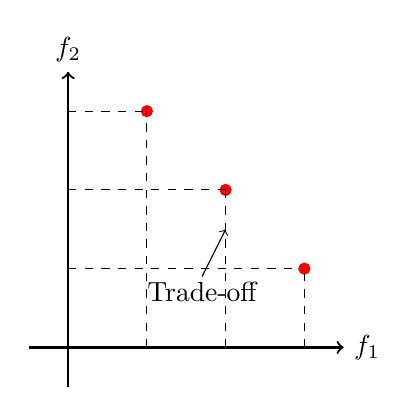
\begin{tikzpicture}
\draw[->,thick] (-0.5,0) -- (3.5,0) node[right] {$f_1$};
\draw[->,thick] (0,-0.5) -- (0,3.5) node[above] {$f_2$};
\filldraw[red] (1,3) circle (2pt);
\filldraw[red] (2,2) circle (2pt);
\filldraw[red] (3,1) circle (2pt);
\draw[dashed] (1,0) -- (1,3);
\draw[dashed] (0,3) -- (1,3);
\draw[dashed] (2,0) -- (2,2);
\draw[dashed] (0,2) -- (2,2);
\draw[dashed] (3,0) -- (3,1);
\draw[dashed] (0,1) -- (3,1);
\node at (1.7,0.7) {Trade-off};
\draw[->] (1.7,0.9) -- (2,1.5);
\end{tikzpicture}
\caption{Pareto çözümleri arasındaki trade-off analizi}
\end{marginfigure}


\subsection{Çok Amaçlı Optimizasyonda Performans Metrikleri}
\subsubsection{Hypervolume (Hiperhaciim)}
Hiperhacim, çok amaçlı optimizasyon algoritmalarının performansını değerlendirmek için kullanılan en yaygın metriklerden biridir. Bu metrik, Pareto cephesinin referans noktasına göre kapladığı alanın veya hacmin ölçüsünü ifade eder. Daha yüksek hiperhacim değeri, algoritmanın daha iyi bir Pareto cephesi bulduğunu gösterir, çünkü bu durum çözüm uzayının daha geniş bir bölümünün kapsandığını ifade eder.

\subsubsection{IGD (Ters Nesil Mesafesi)}
Ters Nesil Mesafesi (IGD), gerçek Pareto cephesi ile algoritma tarafından bulunan çözüm kümesi arasındaki mesafenin bir ölçüsüdür. Bu metrik, bulunan çözümlerin gerçek Pareto cephesine ne kadar yakın olduğunu ve cepheyi ne kadar iyi temsil ettiğini gösterir. Daha düşük IGD değeri, algoritmanın gerçek Pareto cephesine daha yakın ve daha iyi dağılmış çözümler bulduğunu ifade eder.

\subsubsection{Yayılım (Çeşitlilik)}
Yayılım metriği, çözüm kümesindeki noktaların birbirlerine olan uzaklığının ölçüsüdür ve Pareto cephesi boyunca çözümlerin ne kadar homojen dağıldığını gösterir. Bu metrik, algoritmanın çözüm uzayını ne kadar iyi keşfettiğini ve çeşitli alternatifler sunabildiğini değerlendirir. Düzgün dağılmış bir Pareto cephesi için daha düşük yayılım değerleri tercih edilir.

\subsubsection{Hesaplama Süresi}
Hesaplama süresi, bir algoritmanın çözüme ulaşmak için harcadığı zamanı ölçer. Bu metrik, algoritmanın verimliliğini ve pratik uygulamalardaki kullanılabilirliğini değerlendirmek için önemlidir. Özellikle karmaşık mühendislik problemlerinde, makul bir sürede iyi sonuçlar verebilen algoritmalar tercih edilir. Hesaplama süresi, algoritmanın karmaşıklığına, problem boyutuna ve uygulama ortamına bağlı olarak değişebilir. \sidenote{Bu parametre oldukça bağıl olması sebebiyle, her zaman güvenilir sonuçlar vermez. Günümüzde CPU Time gibi daha modern metrikler kullanılır.}